\documentclass[11pt]{standalone}

\usepackage{helvet}

\usepackage{ifthen}
\usepackage{tikz} 
\usetikzlibrary{shapes.misc}
\usetikzlibrary{arrows,arrows.meta}
\usetikzlibrary{calc,intersections, patterns, math}

\definecolor{pfeil}{RGB}{168,167,167}
\definecolor{petrol}{RGB}{0, 118, 136}
\definecolor{darkgoldenrod}{RGB}{184, 134, 11}
\colorlet{petrol-lighter}{petrol!40}
\colorlet{darkgoldenrod-lighter}{darkgoldenrod!40}

\begin{document}

\def\scl{0.25}

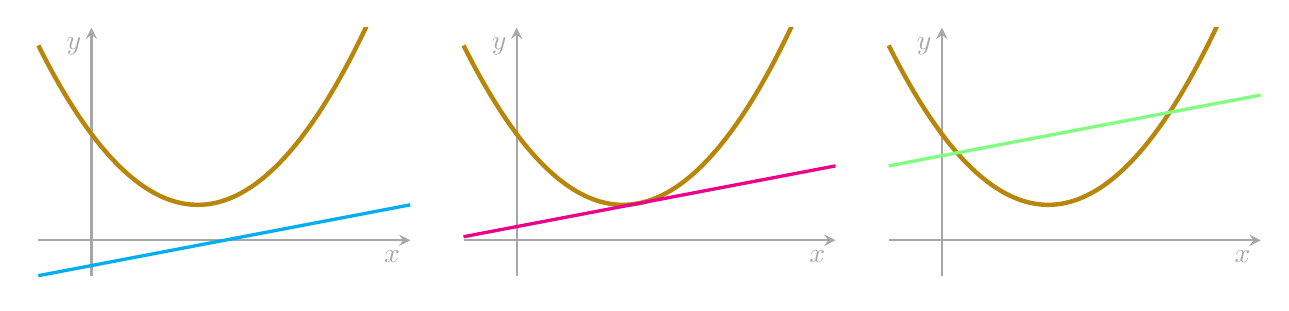
\begin{tikzpicture}[pfeil, scale=0.9,>=stealth] % , scale=\scl
	

    % \draw[thick, fill=petrol!20, draw=petrol-lighter, rounded corners=2ex, opacity=0.5] (0,0) rectangle ++ (1.5,3.5);
    % \draw[thick, fill=darkgoldenrod!20, draw=darkgoldenrod-lighter, rounded corners=2ex, opacity=0.5] (5,0) rectangle ++ (1.5,3.5);

	\begin{scope}[xscale=1.5]
		\begin{scope}
			\clip(-0.6,-0.6) rectangle (3,3);
			\draw[thick,-stealth] (-0.5,0)--(3,0) node[below left]{$x$};
			\draw[thick,-stealth] (0,-0.5)--(0,3) node[below left]{$y$};
			\draw[darkgoldenrod,smooth,domain=-0.5:3,samples=50,ultra thick] plot (\x,{(\x-1)^2+0.5});
			
			\draw[cyan, very thick] (-0.5,-0.5) -- (3,0.5);
		\end{scope}

		\begin{scope}[xshift = 4cm]
			\clip(-0.6,-0.6) rectangle (3,3);
			\draw[thick,-stealth] (-0.5,0)--(3,0) node[below left]{$x$};
			\draw[thick,-stealth] (0,-0.5)--(0,3) node[below left]{$y$};
			\draw[darkgoldenrod,smooth,domain=-0.5:3,samples=50,ultra thick] plot (\x,{(\x-1)^2+0.5});
			
			\draw[magenta, very thick] (-0.5,-0.5+0.55) -- (3,0.5+0.55);
		\end{scope}

		\begin{scope}[xshift=8cm]
			\clip(-0.6,-0.6) rectangle (3,3);
			\draw[thick,-stealth] (-0.5,0)--(3,0) node[below left]{$x$};
			\draw[thick,-stealth] (0,-0.5)--(0,3) node[below left]{$y$};
			\draw[darkgoldenrod,smooth,domain=-0.5:3,samples=50,ultra thick] plot (\x,{(\x-1)^2+0.5});
			
			\draw[green!50!white, very thick] (-0.5,-0.5+1.55) -- (3,0.5+1.55);
		\end{scope}


	\end{scope}

	

\end{tikzpicture}

\end{document}
